\part{Optimeringsproblemer og Optimalitet}
\label{part:introduction}
\chapter{Forhåndskunnskaper}
\label{chap:mathematical_background}

\section{Vektorrom og produkter}

\subsection{Ytre og indre produkter}
\begin{definition}{Ytre produkt}{outer_product}
	Gitt to vektorer \( \symbf{a} \in \R^m \) og \( \symbf{b} \in \R^n \), er det ytre produktet definert som:
	\[
		\symbf{a} \otimes \symbf{b} = \symbf{a} \symbf{b}^\top =
		\begin{bmatrix}
			a_1b_1 & a_1b_2 & \cdots & a_1b_n \\
			a_2b_1 & a_2b_2 & \cdots & a_2b_n \\
			\vdots & \vdots & \ddots & \vdots \\
			a_mb_1 & a_mb_2 & \cdots & a_mb_n
		\end{bmatrix}
	\]
\end{definition}

\begin{definition}{Indre produkt}{inner_product}
	Gitt to vektorer \( \symbf{a}, \symbf{b} \in \R^n \), er det indre produktet definert som:

	\[
		\symbf{a} \cdot \symbf{b} = \symbf{a}^\top \symbf{b} = \sum_{i=1}^{n} a_i b_i
	\]

\end{definition}

\section{Mengder}

\subsection{Baller}
En åpen ball i \(\R^d\) er en mengde av punkter \(\mathbf{x}\) som ligger innenfor en viss avstand \(r\) fra et sentrum \(\mathbf{x_0}\).

Den er definert ved hjelp av den euklidiske normen \(\norm{\cdot}\), som måler avstanden mellom to punkter i rommet.

\begin{definition}{Åpen Ball}{open_ball}
	En åpen ball \(B(\mathbf{x}_0, r)\) i \(\R^d\) med sentrum \(\mathbf{x_0}\) og radius \(r\) er definert som:
	\[
		B(\mathbf{x}_0, r) = \{ \mathbf{x} \in \R^d : \norm{\mathbf{x} - \mathbf{x}_0} < r\}
	\]
	\begin{itemize}
		\item \(B(\mathbf{x}_0, r)\) er åpen hvis den ikke inkluderer grensen.
		\item \(B(\mathbf{x}_0, r)\) er lukket hvis den inkluderer grensen.
	\end{itemize}
\end{definition}

\subsection{Nivåsett}
Intuitivt er nivåsettet til en funksjon \( f \) i et punkt \( y \) mengden av alle punkter \( x \) som har samme eller lavere verdi enn \( y \) under \( f \).
\begin{definition}{Nivåsett}{level_set}
	\(f: \Omega \to \overline{\R}\) er en funksjon. Vi definerer nivåsettet til \(f\) i punktet \(y \in \R\) som:
	\[
		\mathcal{L}_f(y) = \{x \in \Omega | f(x) = y\}.
	\]
\end{definition}

\subsection{Åpen mengde}

\begin{definition}{Åpen mengde}{open_set}
	En mengde \(A \subset \R^n\) er åpen hvis for alle \(x \in A\) finnes det en \(\varepsilon > 0\) slik at \(B(x, \varepsilon) \subset A\).
	\[
		\forall x \in A, \exists \varepsilon > 0 \text{ s.a. } B(x, \varepsilon) \subset A
	\]
\end{definition}

\subsection{Lukket mengde}
\begin{definition}{Lukket mengde}{closed_set}
	En mengde \(A \subset \R^n\) er lukket hvis komplementet \(A^c\) er åpent.
	\[
		A \text{ er lukket} \Leftrightarrow A^c \text{ er åpen}
	\]
\end{definition}

\subsection{Begrenset mengde}

En mengde er begrenset hvis den ikke strekker seg til uendelig langt i noen retning.
Intuitivt kan vi si at en mengde er begrenset hvis den kan plasseres innenfor en kule med endelig radius.

\begin{definition}{Begrenset mengde}{bounded_set}
	En mengde \(A \subset \R^n\) er begrenset hvis det finnes en \(R > 0\) slik at
	\[
		\norm{x} \leq R \quad \forall x \in A
	\]
\end{definition}

\subsection{Kompakt mengde}

En kompakt mengde er en mengde som er både lukket og begrenset. Dette betyr at den er avgrenset og inneholder alle sine grenseverdier.

\begin{definition}{Kompakt mengde}{compact_set}
	En mengde \(A \subset \R^n\) er kompakt hvis den er lukket og begrenset.
	\[
		A \text{ er kompakt} \Leftrightarrow A \text{ er lukket og begrenset}
	\]
\end{definition}

\section{Funksjoner}
\subsection{Nedre semi-kontinuerlige funksjoner}
En nedre semikontinuerlig funksjon (\textit{lower semi-continuous function}) er en funksjon som ikke har plutselige "hopp nedover".

Tenk deg at du nærmer deg et punkt \( \symbf{x_0} \) fra alle mulige retninger:
\begin{itemize}
	\item Verdien av funksjonen i \( \symbf{x_0} \) vil ikke være høyere enn verdiene du ser når du kommer nærmere.
	\item Funksjonen kan ha "hopp oppover".
\end{itemize}


\begin{definition}{Nedre semi-kontinuerlig funksjoner}{lsc}
	\(f: \Omega (\subset \R^d) \to \overline{\R}\) være en funksjon. Vi sier at \(f\) er nedre semi-kontinuerlig (lsc) i punktet \(x_0\) hvis for alle \(\varepsilon > 0\) finnes det en \(\delta > 0\) slik at
	\[
		f(x) > f(x_0) - \varepsilon \quad \text{for alle} \quad x \in B(x_0, \delta).
	\]
	\begin{enumerate}
		\item \(f\) er (lsc) i \(x_0\) hvis det for alle \(\alpha \in \R\) er mengden \(\mathcal{L}_f(\alpha) = \{x | f(x) < \alpha \} \text{ er åpen i } \R^d\)
		\item \(f\) er (lsc) i \(x_0 \in X\) hvis og bare hvis: \(\liminf_{x \to x_0} f(x) \geq f(x_0)\).
	\end{enumerate}
\end{definition}
\begin{example}{Eksempel på en nedre semi-kontinuerlig funksjon}{lsc}
	\includegraphics[width=0.5\textwidth]{figures/example_lsc.png}
\end{example}

\subsection{Koersivitet}
En koersiv funksjon er intuitivt en funksjon som "går mot uendelig" når vi beveger oss mot kanten av definisjonsmengden hvor \( f \) er definert.

\begin{definition}{Koersivitet}{coercive}
	En funksjon \(f: \Omega \to \R\) er koersiv hvis for alle \(y \in \R\) er nivåmengden \(\mathcal{L}_f(y) = \{x \in \Omega | f(x) \leq y\}\) kompakt.

	\[
		\lim_{\norm{x} \to +\infty} f(x) = +\infty
	\]
\end{definition}

\subsection{Konveksitet, kvasi-konveksitet og konvekse mengder}

Konveksitet er et viktig begrep i optimering og matematikk generelt. Det refererer til formen på en funksjon eller en mengde.
\begin{itemize}
	\item En konveks funksjon har en bue som vender oppover.
	\item En konkav funksjon har en bue som vender nedover.
	\item En konveks mengde er en mengde der enhver linje mellom to punkter i mengden også ligger helt innenfor mengden.
\end{itemize}

\begin{definition}{Konveks funksjon}{convex_function}
	En funksjon \(f: \R^n \to \R\) er konveks hvis for alle \(x, y \in \R^n\) og \(\lambda \in [0, 1]\) har vi:

	\begin{align*}
		f(\lambda x + (1 - \lambda)y) & \leq \lambda f(x) + (1 - \lambda)f(y) \\
	\end{align*}
\end{definition}

\begin{definition}{Strengt konveks funksjon}{strictly_convex}
	En funksjon \(f: \R^n \to \R\) er strengt konveks hvis for alle \(x, y \in \R^n\) og \(\lambda \in (0, 1)\) har vi:
	\[
		f(\lambda x + (1 - \lambda)y) < \lambda f(x) + (1 - \lambda)f(y)
	\]
\end{definition}

\begin{remark}{Konveksitet med indre-produkt notasjon}{convex_inner_product}
	En funksjon  \(f: \R^n \to \R\) er konveks hvis og bare hvis:
	\[
		f(y) - f(x) \geq  \langle \nabla f(x), y - x \rangle
	\]
	for alle  \(x, y \in \R^n\).
\end{remark}


\begin{remark}{Kvasi-konveks}{quasi_convex}
	En funksjon \(f: \R^d \to \R\) er kvasi-konveks hvis for alle \(x, y \in \R^n\) og \(\lambda \in (0, 1)\) har vi:

	\[
		f(\lambda x + (1 - \lambda)y) \leq \max\{f(x), f(y)\}
	\]

	En alternativ definisjon er at en funksjon er kvasi-konveks hvis alle nivåsettene er konvekse.

	\[
		\mathcal{L}_f(y) = \{x \in \R^n | f(x) \leq y\} \quad \text{er konveks for alle} \quad y \in \R
	\]

	\[
		\boxed{\underbrace{\forall \alpha \in \R, \mathcal{L}_f(\alpha) \text{ er konveks}}_{f \text{ er kvasi-konveks }}\Longleftrightarrow \forall x, y \in \R^d,\lambda \text{ s.a. } f(\lambda x + (1-\lambda)y) \leq \max \{ f(x), f(y) \}}
	\]
\end{remark}

\begin{definition}{Konveks sett}{convex_set}
	En mengde \(C \subset \R^n\) er (strengt) konveks når:

	\begin{align*}
		\lambda x + (1 - \lambda)y & \in C \quad \forall \; x, y \in C, \lambda \in [0, 1] \tag{Konveks}                   \\
		\lambda x + (1 - \lambda)y & \in C \quad \forall \; x, y \in C, \lambda \in (0, 1), x \neq y \tag{Strengt konveks}
	\end{align*}

\end{definition}

\begin{definition}{Konveks kombinasjon}{convex_combination}
	En konveks kombinasjon av punkter $x_1, x_2, \ldots, x_n$ i $\mathbb{R}^d$ er ethvert punkt på formen:
	\[
		\sum_{i=1}^n \lambda_i x_i \quad \text{der} \quad \lambda_i \geq 0, \sum_{i=1}^n \lambda_i = 1
	\]
\end{definition}

\begin{remark}{Karakterisering av deriverbare konvekse funksjoner}{convex-characterization}
	For en deriverbar funksjon  \(f: \R^n \to \R\) er følgende ekvivalente:
	\begin{itemize}
		\item  \(f\) er konveks
		\item For alle  \(x, y \in \R^n\) gjelder:
		      \[
			      f(y) \geq f(x) + \nabla f(x)^\top (y - x)
		      \]
	\end{itemize}
\end{remark}

\section{Geometriske objekter}
\subsection{Simplex}
Et simplex er en geometrisk figur som kan forstås som den enkleste formen i et gitt antall dimensjoner. For eksempel er et 0-simplex et punkt, et 1-simplex er en linje, et 2-simplex er en trekant, og så videre.

\begin{definition}{Simplex}{simplex}
	Et simplex i \( \mathbb{R}^n \) er et \( n \)-dimensjonalt objekt laget av \( n+1 \) punkter (hjørner) som ikke ligger i samme hyperplan.

	\begin{figure}[H]
		\centering
		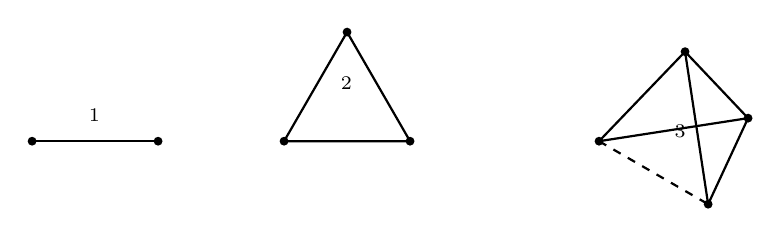
\begin{tikzpicture}[scale=0.8]
			% R1 simplex (line)
			\begin{scope}[shift={(-4,0)}]
				\draw[thick] (0,0) -- (2,0);
				\fill (0,0) circle (2pt);
				\fill (2,0) circle (2pt);
				\node[above] at (1,0) {$\R^1$};
			\end{scope}

			% R2 simplex (triangle)
			\begin{scope}[shift={(0,0)}]
				\draw[thick] (0,0) -- (2,0) -- (1,1.732) -- cycle;
				\fill (0,0) circle (2pt);
				\fill (2,0) circle (2pt);
				\fill (1,1.732) circle (2pt);
				\node[above] at (1,0.5) {$\R^2$};
			\end{scope}

			% R3 simplex (tetrahedron)
			\begin{scope}[shift={(5,0)}, x={(0.866cm,-0.5cm)}, y={(0.866cm,0.5cm)}, z={(0cm,1cm)}]
				% Back triangle
				\draw[thick,dashed] (0,0,0) -- (2,0,0);
				\draw[thick] (2,0,0) -- (1,1.732,0) -- (0,0,0);
				% Vertical edges to top point
				\draw[thick] (0,0,0) -- (1,0.577,1.633);
				\draw[thick] (2,0,0) -- (1,0.577,1.633);
				\draw[thick] (1,1.732,0) -- (1,0.577,1.633);
				% Points
				\fill (0,0,0) circle (2pt);
				\fill (2,0,0) circle (2pt);
				\fill (1,1.732,0) circle (2pt);
				\fill (1,0.577,1.633) circle (2pt);
				\node[above] at (1,0.5,0) {$\R^3$};
			\end{scope}
		\end{tikzpicture}
		\caption{Simplex i ulike dimensjoner.}
	\end{figure}
\end{definition}

\chapter{Hva er optimering?}
\label{chap:what_is_optimization}

Optimering er et felt innen matematikken som handler om å finne den beste løsningen på et gitt problem, enten med eller uten restriksjoner på løsningsrommet.

Målet i et \emph{optimeringsproblem} er å finne en variabel \(x^\star \in \Omega\) som minimerer eller maksimerer en gitt funksjon \(f: \Omega \to \R\), 
kalt \emph{mål\-funksjonen} eller \emph{kostnads\-funksjonen}.

\section{Optimeringsproblemer i \texorpdfstring{\(\R^d\)}{Rd}}

Mengden \(\Omega \subseteq \R^d\) betegner de tillatte løsningene og kalles ofte \emph{søkeområdet} eller den \emph{tillatte mengden (eng. feasible set)}.

\begin{definition}{Optimeringsproblemet \((P)\)}{def:optimization_problem}

	La \(f: \Omega \to \R\) være en funksjon vi ønsker å minimere eller maksimere, der \(\Omega \subseteq \R^d\) er mengden av tillatte (mulige) løsninger.
	\[
		\min_{x \in \Omega} f(x) \quad \text{eller} \quad \max_{x \in \Omega} f(x) \tag{P}
	\]

\end{definition}

Vi fokuserer hovedsakelig på minimeringsproblemer, siden maksimeringsproblemer enkelt kan omformuleres ved å erstatte \(f(x)\) med \(-f(x)\). 
De fleste algoritmene vi diskuterer, er designet for å løse minimeringsproblemer.

\section{Ubundet og Bundet optimering}
Ulike problemtyper oppstår ut fra hvordan denne mengden \(\Omega\) er definert, og hvilke egenskaper funksjonen \(f\) har. Nedenfor gir vi en oversikt over de mest sentrale klassene av optimeringsproblemer:

\begin{itemize}
	\item \textbf{Ubundet optimering}: Dette er den enkleste typen, uten eksplisitte restriksjoner på variabelen \(x\). Her er \(\Omega = \R^d\), og vi søker å minimere \(f(x)\) over hele rommet.
	\item \textbf{Betinget optimering}: Her pålegges løsningen restriksjoner, og den tillatte mengden \(\Omega \subset \R^d\) er definert ved:
	\[
		\Omega = \{ x \in \R^d \mid g_i(x) \leq 0, \, i \in \mathcal{I}, \quad h_j(x) = 0, \, j \in \mathcal{E} \}.
	\]
	\begin{itemize}
		\item \textbf{Lineær programmering (LP)}: Når \(f\) og restriksjonene er lineære.
		\item \textbf{Ikke-lineær programmering (NLP)}: Når én eller flere av \(f\), \(g_i\), eller \(h_j\) er ikke-lineære.
		\item \textbf{Kvadratisk programmering (QP)}: Når \(f\) er kvadratisk og restriksjonene er lineære.
	\end{itemize}
	\item \textbf{Konveks optimering}: En spesialklasse der \(f\) og \(\Omega\) er konvekse. 
	Dette forteller oss at enhver lokal løsning er global, løsningen er entydig hvis \(f\) er strengt konveks, og effektive algoritmer finnes.
\end{itemize}

\section{Globale og lokale løsninger}
\label{sec:global_and_local_solutions}
I optimeringsproblemer er det viktig å skille mellom globale og lokale løsninger. En global løsning er den beste løsningen i hele søkeområdet, mens en lokal løsning er den beste løsningen i et begrenset område rundt et punkt.


\subsection{Globale løsninger}
En global løsning er den beste løsningen i hele søkeområdet \(\Omega\). Dette betyr at det ikke finnes noen annen løsning i hele \(\Omega\) som gir en bedre verdi for funksjonen \(f\).

\begin{definition}{Globale løsninger}{global_solution}

	\medskip
	For en funksjon \(f: \Omega \to \R\) sier vi at \(\symbf{x}^\star \in \Omega\) er en global løsning av minimeringsproblemet~\eqref{eq:global_minimization_problem} hvis:

	\begin{align*}
		f(\symbf{x}^\star) & \leq f(\symbf{x}) \quad \forall \symbf{x} \in \Omega \tag{Global}                                      \\
		f(\symbf{x}^\star) & < f(\symbf{x}) \quad \forall \symbf{x} \in \Omega, \symbf{x} \neq \symbf{x}^\star \tag{Strengt Global}
	\end{align*}
\end{definition}

\subsubsection{Eksistens av globale løsninger}

En funksjon \(f: \Omega \subset \R^d \to \overline{\R}\) har en global løsning (minimum) i \(\Omega\) hvis den er:

\begin{itemize}
	\item \textbf{Nedre semi-kontinuerlig}: For alle \(x \in \Omega\) og alle sekvenser \((x_n)\) som konvergerer mot \(x\):
	      \[
		      f(x) \leq \liminf_{n \to \infty} f(x_n).
	      \]
	\item \textbf{Koersiv}: Det finnes en konstant \(M > 0\) slik at
	      \[
		      f(x) \geq M \quad \forall x \in \Omega.
	      \]
	      Dette sikrer at \(f\) ikke går mot \(-\infty\) når \(x\) går mot uendelig.
\end{itemize}

\begin{theorem}{Eksistens av globale løsninger}{existence_of_global_solution}
	La \(f: \Omega \subset \R^d \to \overline{\R}\) være nedre semi-kontinuerlig og koersiv på \(\Omega\). Da har \(f\) en global løsning (minimum) i \(\Omega\).
\end{theorem}

\subsection{Lokale løsninger}
En lokal løsning er den beste løsningen i et begrenset område rundt et punkt \(\symbf{x}^\star\).
For å avgjøre om \(\symbf{x}^\star\) er en lokal løsning, må vi undersøke om det finnes bedre løsninger i nærheten. 
De fleste metoder for dette baseres på Taylor-utvikling \ref{thm:taylor_theorem}.


\begin{definition}{Lokal løsning}{}
	La \(f: \Omega \to \R\) være en funksjon.

	Vi sier at \(x^\star \in \Omega\) er en lokal løsning av optimeringsproblemet hvis, for en viss \(\varepsilon > 0\):

	\begin{align*}
		f(\symbf{x}^\star) & \leq f(\symbf{x}) \quad \forall \; \symbf{x} \in B(\symbf{x}^\star, \varepsilon) \cap \Omega,                                                  \\
		f(\symbf{x}^\star) & < f(\symbf{x}) \quad \forall \; \symbf{x} \in B(\symbf{x}^\star, \varepsilon) \cap \Omega, \symbf{x} \neq \symbf{x}^\star. \tag{Strengt lokal}
	\end{align*}

	hvor \(B(\symbf{x}^\star, \varepsilon)\) er en åpen kule med sentrum \(\symbf{x}^\star\) og radius \(\varepsilon\)~\ref{def:open_ball}.
\end{definition}

\subsubsection{Taylors teorem}
Taylor-utvikling er en metode for å tilnærme en funksjon ved hjelp av dens deriverte.
Den gir oss en måte å uttrykke funksjonen som en sum av dens verdier og deriverte i et punkt, noe som kan være nyttig for å analysere oppførselen til funksjonen i nærheten av det punktet.

Ved hjelp av Taylor-utvikling kan vi avgjøre om \(\symbf{x}^\star\) er en lokal løsning ved å sjekke om gradienten \(\nabla f(\symbf{x}^\star) = 0\) og Hesse-matrisen \(\nabla^2 f(\symbf{x}^\star)\)

\begin{theorem}{Taylors teorem}{taylors_theorem}
	Anta at \(f: \R^n \to \R\) med \(\mathbf{p}\in\R^n\), og la \(t\in[0,1]\).

	\medskip

	Hvis \(f\in\Ccal^1\) (én gang kontinuerlig deriverbar):
	\[
		f(\mathbf{x} + \mathbf{p}) = f(\mathbf{x}) + \nabla f(\mathbf{x}+t\mathbf{p})^\top \mathbf{p},
	\]

	Hvis \(f \in \Ccal^2\) (to ganger kontinuerlig deriverbar):

	\begin{align*}
		\nabla f(\mathbf{x} + \mathbf{p}) = \nabla f(\mathbf{x}) + \int_0^1 \nabla^2 f(\mathbf{x}+t\mathbf{p})\mathbf{p} dt, \\
		\boxed{f(\mathbf{x} + \mathbf{p}) = f(\mathbf{x}) + \nabla f(\mathbf{x})^\top \mathbf{p} + \frac{1}{2}\mathbf{p}^\top \nabla^2 f(\mathbf{x}+t\mathbf{p})\mathbf{p}}
	\end{align*}
\end{theorem}

\subsubsection{Isolerte lokale løsninger}
En isolert lokal løsning er en lokal løsning der det ikke finnes andre løsninger i nærheten. Dette betyr at det er en viss avstand fra \(\symbf{x}^\star\) til alle andre løsninger.

\begin{lemma}{Isolert lokal løsning}{isolated_local_solution}
	La \(f: \Omega \to \R\) være en funksjon.

	Hvis \(\symbf{x}^\star \in \Omega\) er en isolert lokal løsning, finnes det en \(\varepsilon > 0\) slik at:

	\[
		f(\symbf{x}^\star) \leq f(\symbf{x}) \quad \forall \; \symbf{x} \in B(\symbf{x}^\star, \varepsilon) \cap \Omega, \symbf{x} \neq \symbf{x}^\star.
	\]
\end{lemma}

\chapter{Optimalitetsbetingelser}
\label{chap:optimality_conditions}
\section{Første Ordens Nødvendige Betingelser}

For en lokal løsning \(\mathbf{x}^\star\) må gradienten være null:

\begin{theorem}{First-Order Necessary Conditions}{first_order_necessary_conditions}
	Hvis \(\mathbf{x}^\star\) er et lokalt minimum, og \(f\) er kontinuerlig deriverbar rundt \(\mathbf{x}^\star\), da er:
	\[
		\nabla f(\mathbf{x}^\star) = 0.
	\]
\end{theorem}

\section{Andre Ordens Nødvendige Betingelser}

For en lokal løsning må både gradienten være null og Hesse-matrisen positiv definit:

\begin{theorem}{Second-Order Necessary Conditions}{second_order_necessary_conditions}
	Hvis \(\mathbf{x}^\star\) er et lokalt minimum, og \(f\) er to ganger kontinuerlig deriverbar rundt \(\mathbf{x}^\star\), da er:
	\[
		\nabla f(\mathbf{x}^\star) = 0 \quad \text{og} \quad \nabla^2 f(\mathbf{x}^\star) \succeq 0.
	\]
\end{theorem}

\section{Andre Ordens Tilstrekkelige Betingelser}

\begin{theorem}{Second-Order Sufficient Conditions}{second_order_sufficient_conditions}
	Hvis \(\nabla f(\mathbf{x}^\star) = 0\) og \(\nabla^2 f(\mathbf{x}^\star) \succ 0\) (positiv definit), da er \(\mathbf{x}^\star\) et \emph{strengt lokalt minimum}.

	\medskip

	Det vil si at det finnes en \(\varepsilon > 0\) slik at:
	\[
		f(\mathbf{x}^\star) < f(\mathbf{x})  \quad \forall \; \mathbf{x} \in B(\mathbf{x}^\star, \varepsilon) \cap \Omega, \mathbf{x} \neq \mathbf{x}^\star.
	\]
\end{theorem}

\section{Stasjonære punkter}
Stasjonære punkter er punkter der gradienten til funksjonen er null. Dette betyr at det ikke er noen retning der funksjonen øker eller minker, og det kan være et minimum, maksimum eller et sadelpunkt.

\begin{definition}{Stasjonære punkter}{stationary_points}
	La \(f: \Omega \to \R\) være en funksjon. Et punkt \(\symbf{x}^\star \in \Omega\) er et stasjonært punkt hvis:
	\[
		\nabla f(\symbf{x}^\star) = 0.
	\]
	Dette betyr at gradienten til \(f\) i punktet \(\symbf{x}^\star\) er lik null.
\end{definition}

\subsection{Konvergens til stasjonære punkter}
Når vi bruker iterative metoder for å finne minimum av en funksjon \(f\), ønsker vi å vite om algoritmen vil konvergere til det stasjonære punktet \(\symbf{x}^\star\).

\begin{theorem}{Konvergens til stasjonære punkter}{convergence_to_stationary_points}
	Anta at \(f: \R^d \to \R\) er en kontinuerlig deriverbar funksjon, og at følgende betingelser er oppfylt:
	\begin{enumerate}
		\item \(\Omega\) er en lukket og begrenset mengde.
		\item \(f(\symbf{x})\) er koersiv.
		\item \(f(\symbf{x})\) er nedre semi-kontinuerlig.
		\item \(\nabla f(\symbf{x})\) eksisterer og er Lipschitz-kontinuerlig.
		\item \(\nabla^2 f(\symbf{x})\) eksisterer og er Lipschitz-kontinuerlig.
	\end{enumerate}
	Da konvergerer sekvensen \((\symbf{x}_k)\) generert av en optimaliseringsalgoritme til et stasjonært punkt \(\symbf{x}^\star\) i \(\Omega\).
	\[
		\lim_{k \to \infty} \|\nabla f(\symbf{x}_k)\| = 0.
	\]
	
	hvor \(\symbf{x}_k\) er iteratene generert av en optimaliseringsalgoritme, og \(\symbf{x}^\star\) tilfredsstiller de førsteordens nødvendige betingelsene \(\nabla f(\symbf{x}^\star) = 0\).

\end{theorem}

\section{Optimalitet og konveksitet}
\label{sec:optimality_and_convexity}
For en konveks funksjon \(f\) er det stasjonære punktet \(\mathbf{x}^\star\) også et globalt minimum. Dette er en viktig egenskap ved konvekse funksjoner, og det gjør dem spesielt nyttige i optimering.

\begin{remark}{Konveksitet og stasjonære punkter}{convexity_and_stationary_points}
	\begin{itemize}
		\item Hvis \(f\) er \textbf{konveks} så er alle lokale minimum \(\mathbf{x}^\star\) også globale minimum.
		\item Hvis \(f\) er \textbf{konveks} og \textbf{deriverbar} så er alle stasjonære punkter \(\mathbf{x}^\star\) også globale minimum.
	\end{itemize}
\end{remark}

\begin{example}{Eksistens og optimalitet}{}
		For \( f(x) = x^2 + 2x \), som er kontinuerlig og koersiv, finnes et globalt minimum i \( x^* = -1 \) der \( f(-1) = -1 \).
\end{example}
\begin{example}{Eksistens og optimalitet}{}
			
	For \( f(x) = x^2 \), har vi \( \nabla f(x) = 2x \). I \( x^* = 0 \) er \( \nabla f(0) = 0 \) og \( \nabla^2 f(x) = 2 > 0 \), som oppfyller SOSC.

\end{example}




